\documentclass[a4paper,12pt]{article}
\usepackage[utf8]{inputenc}
\usepackage{amsmath, amssymb}
\usepackage{geometry}
\usepackage{graphicx}
\usepackage{pgfplots}
\usepackage{fancyhdr}
\usepackage{hyperref}
\usepackage{titlesec}
\usepackage{graphicx}
\titleformat{\section}
  {\normalfont\Large\bfseries\centering}  % Format: font size, bold, centered
  {\thesection}{1em}{} 
\pagestyle{fancy}
\pgfplotsset{compat=1.18}
\fancyhead{}
\fancyfoot{}
\fancyhead[L]{Gabriele Perna}          % Left side
\fancyhead[C]{Fondamenti di Informatica}     % Center
\fancyhead[R]{2025/2026}             % Right side
\fancyfoot[C]{\thepage}           % Page number in the center of footer
\let\oldsection\section
\renewcommand{\section}{\clearpage\oldsection}
\geometry{margin=2.5cm}

\title{Fondamenti di Informatica}
\author{Gabriele Perna}
\date{}

\begin{document}

\maketitle
\tableofcontents
\section{Insiemi}

\subsection{Definizione}
Un insieme è una collezione di oggetti detti elementi.  
In un insieme non esiste un ordine di elementi e ogni elemento è presente oppure no.  
Non esiste molteplicità degli elementi.

\subsection{Notazioni}
\begin{itemize}
    \item Lettere maiuscole: indicano insiemi ($A$, $B$)
    \item Lettere minuscole: indicano elementi ($a$, $b$)
\end{itemize}

Un insieme vuoto si indica con $\emptyset$.  

Appartenenza: 
\[
a \in A \quad \text{“l'elemento $a$ appartiene all’insieme $A$”}
\]

Definizione tramite parentesi graffe:  
\[
A = \{1,2,3,4,5,11\}
\]

\subsection{Descrizione e rappresentazione degli insiemi}
\begin{itemize}
    \item Per enumerazione: si elencano gli elementi con le parentesi graffe.
    \item Per proprietà: si definiscono le proprietà che gli elementi devono soddisfare.
\end{itemize}

Template: 
\[
A = \{ x \in B \mid P(x) \}
\]
“L’insieme $A$ contiene tutti gli elementi di $B$ che soddisfano la proprietà $P$”.

\subsection{Diagrammi di Eulero-Venn}
Utilizzati per rappresentare graficamente gli insiemi.

\subsection{Uguaglianza e inclusione tra insiemi}
\begin{itemize}
    \item Due insiemi sono uguali se ogni elemento del primo appartiene al secondo e viceversa.
    \item Sottoinsieme: $A \subseteq B$ indica che tutti gli elementi di $A$ appartengono anche a $B$.  
    $A \subset B$ indica che $A$ è sottoinsieme proprio di $B$.
\end{itemize}

\subsection{Disgiunzione}
Due insiemi sono disgiunti se non hanno elementi in comune.

\subsection{Insieme universo}
L’insieme universo $U$ include tutti gli elementi nel contesto considerato.

\subsection{Proprietà di uguaglianza e inclusione}
\begin{itemize}
    \item Riflessività: $A = A$, $A \subseteq A$, $A \subset A$ NON vale
    \item Transitività: se $A=B$ e $B=C$ allora $A=C$; se $A\subseteq B$ e $B\subseteq C$ allora $A\subseteq C$
    \item Simmetria: $A=B \implies B=A$ (valida solo per uguaglianza)
    \item Antisimmetria: $A \subseteq B$ e $B \subseteq A \implies A=B$
\end{itemize}

\subsection{Operazioni tra insiemi}
\begin{itemize}
    \item Unione: $A \cup B = \{x \mid x \in A \vee x \in B\}$
    \item Intersezione: $A \cap B = \{x \mid x \in A \wedge x \in B\}$
    \item Differenza: $A \setminus B = \{x \mid x \in A \wedge x \notin B\}$
    \item Complemento: $\overline{B} = U \setminus B$ o $\neg B$
\end{itemize}

\subsection{Implicazioni logiche}
\begin{align*}
P \Rightarrow Q &\quad \text{“Se $P$ allora $Q$”} \\
P \Leftarrow Q &\quad \text{Conseguenza} \\
P \Leftrightarrow Q &\quad \text{Doppia implicazione}
\end{align*}

\subsection{Tipi di dimostrazione}
\begin{itemize}
    \item Discorsiva: si ricorre alle definizioni
    \item Grafica: si usa un diagramma
    \item Per sostituzione: si applicano leggi per sostituire elementi
\end{itemize}
Alla fine di una dimostrazione confermata si aggiunge $\blacksquare$.

\subsection{Leggi degli insiemi}
\begin{itemize}
    \item Legge di De Morgan: 
    \[
    \overline{A \cup B} = \overline{A} \cap \overline{B}, \quad 
    \overline{A \cap B} = \overline{A} \cup \overline{B}
    \]
\end{itemize}

\subsection{Cardinalità}
La cardinalità di un insieme finito $A$ è il numero dei suoi elementi: $|A| = n$.

\subsection{Insiemi di insiemi}
\begin{align*}
A &= \{\{2,4,5\},\{3,4,1\}\}
\end{align*}

\subsection{Insieme delle parti}
\[
P(A) = \{ x \mid x \subseteq A\}
\]
Esempio: $A=\{1,2,3\} \implies P(A) = \{\emptyset, \{1\}, \{2\}, \{3\}, \{1,2\}, \{1,3\}, \{2,3\}, \{1,2,3\}\}$

\subsection{Famiglie e partizioni di insiemi}
\[
F = \{ A_i \mid i \in I \}, \quad \bigcup F = \bigcup A_i
\]  
Una partizione di $A$ è una famiglia di sottoinsiemi non vuoti, che copre $A$ e sono a due a due disgiunti.

\subsection{Prodotto cartesiano}
Il prodotto cartesiano tra due insiemi $A$ e $B$ è:
\[
A \times B = \{ (a,b) \mid a \in A, b \in B \}
\]

\section{Relazioni tra insiemi}

\subsection{Definizione}
Dati due insiemi $A$ e $B$, una relazione $R$ tra $A$ e $B$ è un sottoinsieme del prodotto cartesiano $A \times B$.  

$A$ è detto \textit{insieme di partenza}, $B$ \textit{insieme di arrivo}.  

Esempio: 
\[
A = \{a,b,c\}, \quad B = \{x,y\}
\] 
\[
R = \{(x,a),(x,c)\} \subseteq A \times B
\] 

Anche la relazione vuota è possibile: 
\[
R = \emptyset \subseteq A \times B
\]

\subsection{Relazione identità}
La relazione identità su un insieme $A$ è: 
\[
\text{Id}_A = \{(x,x) \mid x \in A\}
\]

\subsection{Composizione di relazioni}
Siano $R: A \leftrightarrow B$ e $S: B \leftrightarrow C$.  
La composizione $R;S: A \leftrightarrow C$ è definita come:
\[
R;S = \{(x,z) \in A \times C \mid \exists y \in B : (x,y) \in R \wedge (y,z) \in S \}
\]

Esempio:  
\[
A = \{x,y,z\}, \quad B = \{a,b,c,d\}, \quad C = \{1,2\}
\]  
\[
R = \{(x,a),(y,b),(z,c),(z,d)\}, \quad S = \{(a,1),(a,2),(c,2),(d,2)\}
\]  
Allora $(x,1) \in R;S$.

\subsection{Relazione opposta}
Dati $R: A \leftrightarrow B$, la relazione opposta $R^{op}: B \leftrightarrow A$ è:
\[
R^{op} = \{(y,x) \in B \times A \mid (x,y) \in R \}
\]

\[
(S^{op};R^{op}) = (R;S)^{op}
\]

\subsection{Proprietà delle relazioni (TUSI)}

\subsubsection{Relazioni totali}
$R: A \leftrightarrow B$ è totale se:
\[
\forall a \in A, \exists b \in B : (a,b) \in R
\]

\subsubsection{Relazioni univalenti}
$R$ è univalente se:
\[
\forall a \in A, \exists \text{ al massimo un } b \in B : (a,b) \in R
\]

\subsubsection{Relazioni suriettive (surgettive)}
$R$ è suriettiva se:
\[
\forall b \in B, \exists a \in A : (a,b) \in R
\]

\subsubsection{Relazioni iniettive}
$R$ è iniettiva se:
\[
\forall b \in B, \exists \text{ al massimo un } a \in A : (a,b) \in R
\]

\subsection{Risultati di dualità}
\[
\text{Se } R \text{ è totale } \iff R^{op} \text{ è suriettiva}
\]  
\[
\text{Se } R \text{ è univalente } \iff R^{op} \text{ è iniettiva}
\]

\subsection{Teorema di caratterizzazione}
\begin{align*}
R \text{ è totale} &\iff \text{Id}_A \subseteq R;R^{op} \\
R \text{ è univalente} &\iff R^{op};R \subseteq \text{Id}_B \\
R \text{ è suriettiva} &\iff \text{Id}_B \subseteq R^{op};R \\
R \text{ è iniettiva} &\iff R;R^{op} \subseteq \text{Id}_A
\end{align*}

\subsection{Composizione e proprietà}
Se due relazioni $R$ e $S$ sono entrambe totali, allora la loro composizione $R;S$ sarà totale.  
Lo stesso vale per univalenza, suriettività e iniettività.

\section{Funzioni}

\subsection{Definizione}
Una funzione è una relazione che è \textbf{totale} e \textbf{univalente}.  

\[
f: A \to B
\]

Ovvero, per ogni elemento $a \in A$ esiste esattamente un elemento $b \in B$ tale che $(a,b) \in f$.  

Esempi di funzioni in informatica sono i connettivi logici.

\subsection{Composizione di funzioni}
Se $f: A \to B$ e $g: B \to C$, allora la composizione è:
\[
f;g: A \to C
\]

\subsection{Funzione parziale}
Una funzione parziale è una funzione che \textbf{non è totale}, quindi è solo equivalente.

\subsection{Biiezione (Bigezione)}
Una funzione $f: A \to B$ che è \textbf{totale}, \textbf{univalente}, \textbf{suriettiva} e \textbf{iniettiva} si chiama \textbf{biiezione}.  

\begin{itemize}
    \item Esiste una corrispondenza $1:1$ tra gli elementi di $A$ e $B$.
    \item Le cardinalità di $A$ e $B$ devono essere uguali.
    \item La relazione identità è una biiezione.
    \item La composizione di due biiezioni è una biiezione.
    \item L'opposta di una biiezione è una biiezione.
\end{itemize}

Se due insiemi sono in biiezione si indica:
\[
A \cong B
\]

\subsection{Teorema di categorizzazione delle biiezioni}
Sia $R: A \leftrightarrow B$. Allora:

\[
R \text{ è biiezione} \iff (\text{Id}_A = R;R^{op}) \wedge (\text{Id}_B = R^{op};R)
\]

\subsection{Proprietà delle biiezioni}
\begin{itemize}
    \item \textbf{Simmetria:} 
    \[
    A \cong B \iff B \cong A
    \]
    \item \textbf{Riflessività:} 
    \[
    A \cong A
    \]
    \item \textbf{Transitività:} 
    \[
    A \cong B \wedge B \cong C \implies A \cong C
    \]
\end{itemize}

\section{Induzione}

Gli insiemi infiniti si definiscono secondo regole di base.  
Tre principali usi dell'induzione:

\begin{enumerate}
    \item Definizione induttiva di insiemi (regole per definire chi appartiene).
    \item Definizione induttiva di funzioni (regole per calcolare $f(A)$).
    \item Dimostrazione di proprietà.
\end{enumerate}

Per definire ognuno di questi si usano delle clausole:

\begin{itemize}
    \item \textbf{Clausola base:} stabilisce il punto di partenza.
    \item \textbf{Clausola induttiva (ipotesi induttiva):} definisce le regole per la propagazione.
    \item \textbf{Clausola terminale:} spesso implicita, indica che solo quanto definito dalle altre due clausole vale.
\end{itemize}

\subsection{Definizione induttiva di un insieme}

\begin{itemize}
    \item Clausola base: certi elementi appartengono ad $A$.
    \item Clausola induttiva: come usare elementi di $A$ per costruirne altri.
    \item Clausola terminale: l'insieme $A$ non contiene altro.
\end{itemize}

\textbf{Esempio:} definizione dei numeri naturali
\[
0 \in \mathbb{N}, \quad n \in \mathbb{N} \implies (n+1) \in \mathbb{N}
\]

\textbf{Esempio:} definizione di $ \mathbb{N} \setminus \{5\} $
\[
0 \in \mathbb{N}, \quad 
n \in \mathbb{N} \wedge n \neq 4 \implies (n+1) \in \mathbb{N}, \quad 
n \in \mathbb{N} \wedge n = 4 \implies (n+2) \in \mathbb{N}
\]

\subsection{Definizione induttiva di una funzione}

\begin{itemize}
    \item Clausola base: definire il valore dell'immagine di alcuni elementi.
    \item Clausola induttiva: dare una regola per calcolare l'immagine degli altri elementi.
\end{itemize}

\textbf{Esempio:} funzione $T: \mathbb{N} \to \mathbb{N}$
\[
T(0) = 0, \quad T(n+1) = T(n) + (n+1)
\]

\[
T(4) = T(3+1) = T(3) + 4 = (T(2) + 3) + 4 = (T(1) + 2 + 3) + 4 = T(0) + 10 = 10
\]

\subsection{Definizione induttiva di una proprietà}

Sia $P(m)$: "$m^2 + m$ è divisibile per 2".  
Vogliamo dimostrare $\forall m \in \mathbb{N}, P(m)$.

\begin{itemize}
    \item Clausola base:
    \[
    P(0) = 0^2 + 0 = 0 \text{ (divisibile per 2)}
    \]
    \item Clausola induttiva: se $m^2 + m$ è divisibile per 2, allora $(m+1)^2 + (m+1)$ è divisibile per 2.
\end{itemize}

\[
(m+1)^2 + (m+1) = m^2 + 2m + 1 + m + 1 = m^2 + m + 2m + 2
\]

Se $m^2 + m = 2k$, allora
\[
(m+1)^2 + (m+1) = 2k + 2m + 2 = 2(k + m + 1)
\]

Divisibile per 2, quindi la proprietà vale.

\section{Relazioni su un insieme}

Sia $R: A \leftrightarrow A \subseteq A \times A$.

\subsection{Proprietà delle relazioni su un insieme (RATSO)}

\begin{itemize}
    \item \textbf{Riflessività:} 
    \[
    \forall a \in A : (a,a) \in R
    \]
    L'identità $Id_A$ e il prodotto cartesiano completo sono riflessivi. Una relazione vuota non lo è.
    
    \item \textbf{Simmetria:} 
    \[
    \forall a,b \in A : (a,b) \in R \implies (b,a) \in R
    \]
    L'identità e il prodotto cartesiano completo sono simmetrici. La relazione vuota è simmetrica.
    
    \item \textbf{Transitività:} 
    \[
    \forall a,b,c \in A : (a,b) \in R \wedge (b,c) \in R \implies (a,c) \in R
    \]
    L'identità e il prodotto cartesiano completo sono transitivi. La relazione vuota è transitiva.
    
    \item \textbf{Anti-simmetria:} 
    \[
    \forall a,b \in A : (a,b) \in R \wedge (b,a) \in R \implies a = b
    \]
    L'identità è anti-simmetrica, il prodotto cartesiano completo non lo è. La relazione vuota è anti-simmetrica.
\end{itemize}

\subsection{Teorema di caratterizzazione}

\begin{itemize}
    \item $R$ è riflessiva $\iff Id_A \subseteq R$
    \item $R$ è simmetrica $\iff R \subseteq R^{op}$ (oppure $R = R^{op}$)
    \item $R$ è transitiva $\iff R;R \subseteq R$
    \item $R$ è anti-simmetrica $\iff R \cap R^{op} \subseteq Id_A$
\end{itemize}

\subsection{Chiusure di una relazione}

\begin{itemize}
    \item \textbf{Chiusura riflessiva:} $R \cup Id_A$
    \item \textbf{Chiusura simmetrica:} $R \cup R^{op}$
    \item \textbf{Chiusura transitiva:} 
    \[
    R^+ = R \cup R^2 \cup R^3 \cup \dots \cup R^n, \quad n = |A|
    \]
    \item \textbf{Chiusura transitiva unita all'identità (Stella di Kleene):} 
    \[
    R^* = R^+ \cup Id_A
    \]
\end{itemize}

\subsection{Relazioni particolari}

\begin{itemize}
    \item \textbf{Relazione di equivalenza:} riflessiva, simmetrica e transitiva (es. $Id_A$, non vuota, prodotto cartesiano)
    \item \textbf{Relazioni di ordinamento parziale:} riflessiva, anti-simmetrica e transitiva (es. $Id_A$, $\leq$)
\end{itemize}

Una relazione è di ordinamento se soddisfa la proprietà di totalità:
\[
\forall a,b \in A, (a,b) \in R \text{ oppure } (b,a) \in R
\]

\section{Grafi orientati}

\subsection{Definizione}

Un grafo orientato è una relazione $E: V \leftrightarrow V$ su un insieme finito $V$:

\begin{itemize}
    \item $V$: insieme dei nodi o vertici
    \item $E$: insieme degli archi
\end{itemize}

\textbf{Proprietà:}
\begin{itemize}
    \item Nodi connessi da un arco sono \textit{adiacenti}
    \item \textit{Vicinato} di un nodo: nodi adiacenti
    \item \textit{Vicinato in entrata}: archi che entrano
    \item \textit{Vicinato in uscita}: archi che partono
    \item Grado in uscita $d^+$, grado in entrata $d^-$
\end{itemize}

\textbf{Hand-shaking Lemma:} 
\[
\sum_{x \in V} d^+(x) = |E|
\]

\subsection{Rappresentazione di grafi orientati}
\paragraph{Matrice di adiacenza:}
$M_ij = M_ji = 1 se {i,j} \in E$\\
\begin{center}
  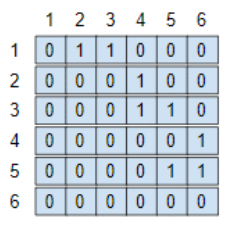
\includegraphics[width=0.5\textwidth]{images/MatriceNonOrientata.png}
\end{center}
\paragraph{Liste di adiacenza:}
\begin{center}
  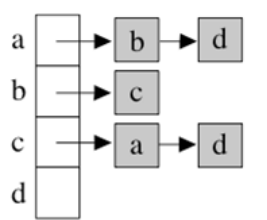
\includegraphics[width=0.5\textwidth]{images/liste.png}
\end{center}

\subsection{Varianti di grafi}

\begin{itemize}
    \item Grafi etichettati e/o pesati: $L: (V \cup E) \to D$
    \item Walk: sequenza di nodi collegati da archi
    \item Trail: walk che non attraversa due volte lo stesso arco
    \item Path: walk che non attraversa due volte lo stesso nodo
    \item Walk chiuso: walk che inizia e finisce allo stesso nodo
    \item Circuito: trail che inizia e finisce nello stesso nodo
    \item Ciclo: path che inizia e finisce sullo stesso nodo
\end{itemize}

\subsection{Connettività}

\begin{itemize}
    \item Grafo orientato fortemente connesso: per ogni $x,y \in V$ esiste un walk da $x$ a $y$
    \item Componente fortemente connessa: sottoinsieme massimale di nodi fortemente connessi
    \item Grafo orientato aciclico (DAG): grafo senza cicli
    \item Nodi con 0 ingressi: sorgenti
    \item Nodi con 0 uscite: pozzi
    \item Arco riflessivo: cappio
\end{itemize}

\subsection{Ordinamento topologico su DAG}

Dato un DAG, un ordinamento topologico è una biiezione $n: V \to \{0,1,2,\dots,|V|-1\}$ tale che
\[
(x,y) \in E \implies n(x) < n(y)
\]

\textbf{Proprietà:}
\begin{itemize}
    \item Ogni DAG ha almeno una sorgente e un pozzo
    \item Ogni sottografo di un DAG è un DAG
    \item Un DAG inverso è comunque un DAG
\end{itemize}

\section{Grafi non orientati}
\subsection{Definizione}
Nei grafi orientati gli archi non sono più orientati e non sono indicati più da frecce, bensì da semplici linee connettive.
Per questo, l'insieme degli archi di un grafo non orientato è un insieme di insiemi di nodi cardinalità 2.
\begin{align*}
P_2(V) = {X \subseteq V : |X| = 2}\\
E \subseteq P_2(V)
\end{align*}
\paragraph{Proprietà}
\begin{itemize}
    \item Un grafo non orientato non può avere cappi.
    \item Nodi \textbf{universali} = connessi a tutti gli altri nodi.
    \item Nodi \textbf{isolati} = non connessi ad alcun nodo.
    \item Walk, trail e path mantengono le stesse definizioni.
    \item Walk chiuso, circuito e ciclo mantengono le stesse definizioni.
    \begin{itemize}
        \item Qui un walk chiuso non implica un circuito, ma un circuito indica un ciclo.
    \end{itemize}
    \item Grafo non orientato connesso = grafo che per ogni coppia di nodi ha un walk.
    \item Componente connessa = insieme massimale di nodi connessi.
    \item Vicinato di $x = N(x) = {y \in V : xy \in E}$
    \item Grado di $x = d_x = |N(x)|$
\end{itemize}

\paragraph{Combinazione di circuiti:}
Se abbiamo due circuiti disgiunti sugli archi ma con almeno un nodo in comune possiamo unirli per formare un circuito unico.


\subsection{Grafo orientato associato a un grafo non orientato}
Se abbiamo un grafo non orientato $G = (V,E)$ e un grafo orientato $\overline{G} = (V,\overline{E})$ allora:
\[
\overline{E} = {(x,y) \in V \times V : {x,y} \in E} : V \leftrightarrow V
\]
\textbf{Hand-shaking Lemma} per i grafi non orientati:
\[
\sum_{x \in V} d^+(x) = 2|E|
\]
\subsection{Rappresentazione di grafi non orientati}
\paragraph{Matrice di adiacenza:}
$M_ij = M_ji = 1 se {i,j} \in E$\\
La diagonale dal vertice in alto a sinistra al vertice in basso a destra sarà sempre vuota dato che non ci sono cappi.
\begin{center}
  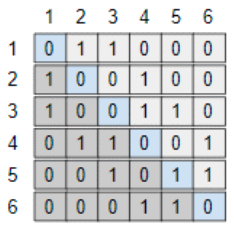
\includegraphics[width=0.5\textwidth]{images/MatriceOrientata.png}
\end{center}
\paragraph{Liste di adiacenza:}
nei grafi non orientati le liste di adiacenza sono più folte, presentando simmetria (se $1$ contiene $4$, allora $4$ contiene $1$)
\begin{center}
  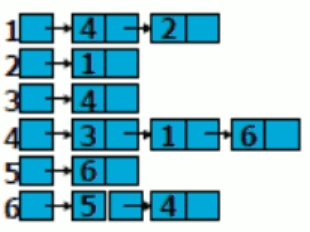
\includegraphics[width=0.5\textwidth]{images/listenonordinate.png}
\end{center}

\section{Alberi}
Un \textbf{albero} è un grafo non orientato, connesso, aciclico e non vuoto.
Gli alberi vengono spessi utilizzati come strutture dati per rappresentare alcune situazioni.
\subsection{Caratteristiche}
\begin{itemize}
    \item Una \textbf{foresta} è un grafo non orientato, aciclico, non vuoto e non connesso.
    \begin{itemize}
        \item Se ad un albero si toglie un arco diventa una foresta.
    \end{itemize}
    \item I nodi alle estremità finali dell'albero (in fondo) si chiamano \textbf{foglie} ed hanno grado 1.
    \item Tutti i nodi con grado $> 1$ si chiamano nodi interni.
    \item Il numero dei path tra due nodi di un albero è sempre 1.
    \item Ogni componente connessa di un albero è un albero.
\end{itemize}

\subsection{Proprietà}
\begin{itemize}
    \item Per ogni coppia di nodi distinti $x,y \in V$ esiste un unico path da x a y.
    \begin{itemize}
        \item Il path in questione esiste perchè è il grafo è connesso ed è unico perche se non fosse unico ci sarebbe un ciclo $\blacksquare$.
    \end{itemize}
    \item Per ogni arco $x,y \in E$ la rimozione di $xy$ rende il grafo non connesso.
    \item Per ogni coppia di nodi distinti $x,y \in V$ tale che $xy \notin E$, l'aggiunta dell'arco $xy$ crea un ciclo.
    \item Ogni albero con almeno due nodi ha almeno una foglia.
    \begin{itemize}
        \item Dalla definizione di albero, un albero è connesso e quindi ogni nodo ha almeno un arco (grado $\ge 1$) e quindi possiamo sicuramente muoverci da un nodo iniziale verso un suo vicino. Se il vicino ha grado 1 è una foglia $\blacksquare$, altrimenti si continua il path fino a quando non si trova la foglia prima di $|V|$ passi.$\blacksquare$
    \end{itemize}
    \item Ogni albero ha esattamente $n-1$ archi con $n = |V|$
    \begin{itemize}
        \item Togliere una foglia mantiene la struttura ad albero e riduce gli archi e i nodi entrambi di 1. \\Per induzione:
        \begin{align*}
            P(0) &= \text{non esistono alberi con 0 nodi} \quad \blacksquare \\
            P(1) &= 0, \text{ esiste solo un tipo di albero con 1 nodo e non può avere archi} \quad \blacksquare \\
            P(n) &\implies P(n+1) \quad \text{per ogni } n+1 \geq 2
        \end{align*}
        L'ipotesi induttiva vale perchè secondo l'osservazione iniziale posso rimuovere una foglia alla volta e mantenere lo stesso rapporto tra archi e nodi.
        Se si continua a rimuovere foglie si ritorna eventualmente al caso base. $\blacksquare$
    \end{itemize}
\end{itemize}

\subsection{Alberi importanti}
\paragraph{Albero radicato: } Un \textbf{albero radicato} ha un nodo speciale chiamato \textbf{root} o \textbf{radice}
\begin{center}
  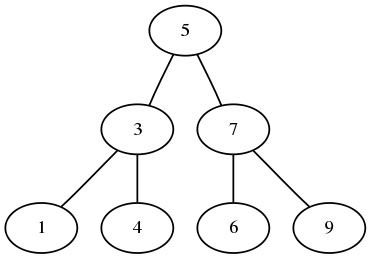
\includegraphics[width=0.5\textwidth]{images/alberoradicato.png}
\end{center}
\paragraph{Alberi ordinali: } i nodi interni hanno un ordinamento totale dei suoi figli.
\paragraph{Alberi cardinali: } i nodi interni hanno $k$ figli che eventualmente possono essere vuoti.
\paragraph{Albero binario di ricerca: } grafo pesato sui nodi, ogni nodo ha al massimo due archi in uscita. Questo tipo di albero ha un ordine da sinitra a destra e permette la ricerca di valori precisi in maniera semplice.
Un albero binario è un albero cardinale con $k = 2$.
\begin{center}
  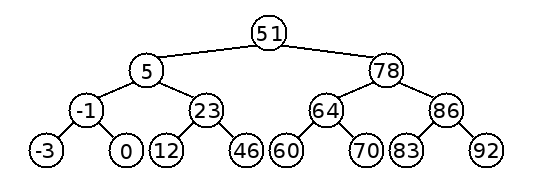
\includegraphics[width=0.5\textwidth]{images/alberobinario.png}
\end{center}
\paragraph{Red-Black Tree: }
\begin{center}
  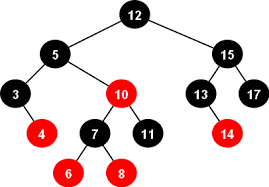
\includegraphics[width=0.5\textwidth]{images/redblacktree.png}
\end{center}
\paragraph{Albero decisionale: } utilizzato spesso nelle AI.
\begin{center}
  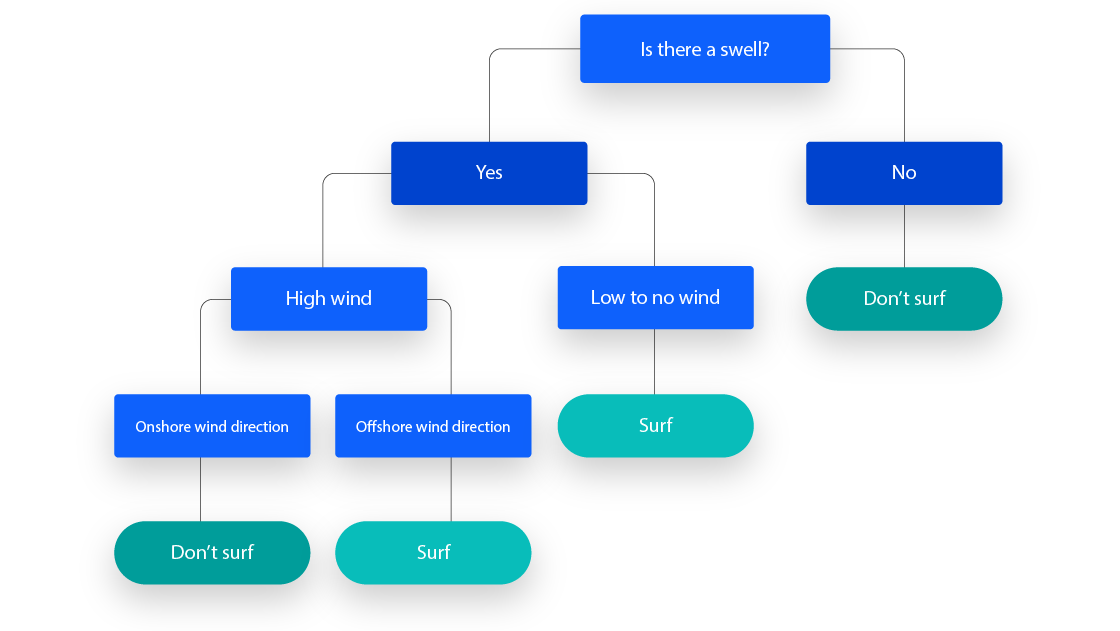
\includegraphics[width=0.5\textwidth]{images/alberodecisionale.png}
\end{center}

\section{Cammini e cicli Euleriani e Hamiltoniani}
\subsection{Teorema di Eulero}
\paragraph{Circuito euleriano: } circuito che passa esattamente una volta per tutti gli archi del grafo.
\paragraph{Trail euleriano (o \emph{percorso euleriano}): } trail che passa esattamente una volta per tutti i nodi del grafo.\\\\
Dato un grafo non orientato e connesso:
\begin{itemize}
    \item Esiste un trail euleriano da $x$ a $y$ se e solo se $x$ e $y$ sono gli unici nodi di grado dispari.
    \begin{itemize}
        \item Se aggiungiamo un nuovo nodo $z$ con archi $zy$ e $zx$ il grafo si trasforma e tutti i nodi avranno adesso un numero pari di archi. Prendiamo il circuito del nuovo grafo ed escludiamo i nuovi archi aggiunti, trovando il trail euleriano.
    \end{itemize}
    \item Esiste un circuito euleriano se e solo se tutti i nodi hanno grado pari.
    \begin{itemize}
        \item Ogni volta che si passa da un nodo ci si entra e poi ci si esce, servono quindi 2 archi ogni volta. Se
        si attraversa tale nodo k volte, serviranno appunto 2k archi. Il secondo arco del nodo da cui si parte si utilizza quando si conclude il circuito.
        \item Un circuito euleriano ovviamente non può esistere se il grafo non è connesso.
    \end{itemize}
\end{itemize}
Dato un grafo orientato e fortemente connesso:
\begin{itemize}
    \item Esiste un ciclo euleriano se e solo se tutti i nodi hanno grado in ingresso uguale al grado in uscita.
    \item Esiste un trail euleriano da x a y se e solo se tutti i nodi hanno grado in ingresso uguale al grado in uscita e $d^+_x = d^-_x + 1$ e $d^-_y = d^+_y + 1$
\end{itemize}

\subsection{Teorema di Hamilton}
Dato un grafo connesso:
\begin{itemize}
    \item un ciclo hamiltoniano è un ciclo che passa esattamente una volta per tutti i nodi del grafo.
    \item un path hamiltoniano è un path che passa esattamente una volta per tutti i nodi del grafo.
\end{itemize}
Non esiste una caratterizzazione semplice come per i ciruciti euleriani, ad oggi non si conosce un algoritmo efficiente ma solo brute-force.

\subsection{Il problema dei sette ponti di Konigsberg}
\begin{center}
  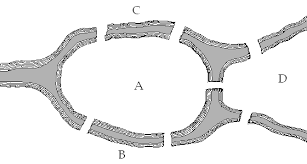
\includegraphics[width=0.5\textwidth]{images/ponti.png}
\end{center}
Il problema dei sette ponti di Königsberg è un famoso problema di topologia e teoria dei grafi, originariamente posto nella città di Königsberg (oggi Kaliningrad). Il problema consiste nel trovare un percorso che attraversi ciascuno dei sette ponti una sola volta e ritorni al punto di partenza.\\
Leonhard Euler dimostrò che tale percorso non esiste, dando così origine alla teoria dei grafi e alla definizione dei \emph{circuiti euleriani}. La sua soluzione si basa sull'analisi dei gradi dei nodi del grafo che rappresenta la città e i suoi ponti.

\subsection{Problema del commesso viaggiatore}
Dato un grafo pesato non orientato, trovare un ciclo hamiltoniano di \textbf{peso minimo}, dove il peso è la somma degli archi attraversati.
\begin{center}
  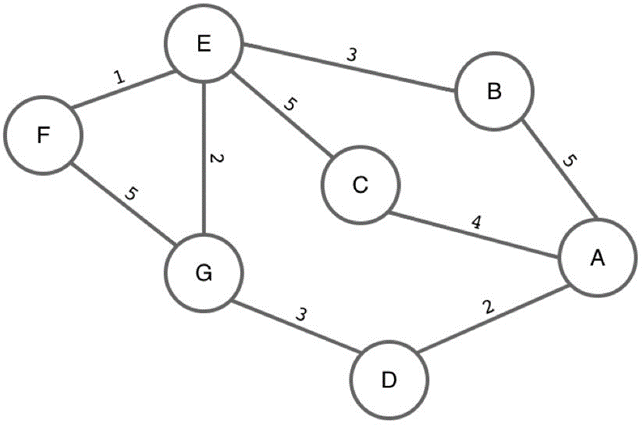
\includegraphics[width=0.5\textwidth]{images/grafopesato.png}
\end{center}

\section{Altro sui grafi}
\paragraph{Diametro di un grafo: } massima distanza tra coppie di nodi.
\paragraph{Profondità di un nodo: } distanza di un nodo dalla radice.
\paragraph{Altezza di un nodo: } massima distanza tra $x$ e le foglie sue discendenti
\paragraph{Altezza di un grafo: } altezza della radice
\paragraph{Uguaglianza tra grafi: } due grafi sono uguali quando hanno gli stessi archi e gli stessi nodi.
\paragraph{Isomorfismo tra grafi: } due grafi hanno la 'stessa forma', a seconda della loro rappresentazione. Espresso
formalmente, esiste una biiezione che mappa i nodi del primo grafo confrontato con quelli del secondo.
\paragraph{Grafo bipartito: } grafo dove ogni nodo corrisponde a un colore (non necessariamente unico) che si distingue dal colore dei suoi vicini. Questo
ovviamente si verifica quando un grafo non ha cicli dispari. Gli alberi sono grafi bipartiti, in quanto basta cambiare colore ad ogni livello.
\paragraph{Spanning Tree: } dato un grafo connesso, uno spanning tree è un albero che connette i nodi del grafo connesso con $n-1$ archi.
\subsection{Distanze}
Una \textbf{distanza} su un insieme A è una funzione $d: A\times A \rightarrow \mathbb{R}$ che soddsfa le seguenti proprietà $\forall x,y,z \in A$
\begin{align*}
    d(x,y) &\geq 0\\
    d(x,y) &= 0 \Longleftrightarrow x = y\\
    d(x,y) &= d(y,x)\\
    d(x,y) &\leq d(x,z) + d(z,y)
\end{align*}
Su un grafo non orientato, la distanza tra due nodi è il numero dei passi che il walk minimo effettua da $x$ a $y$.\\
Su un grafo orientato la condizione della simmetria non viene soddisfatta e la regola del walk minimo non vale.

\section{Calcolo combinatorio}
Il \textbf{calcolo combinatorio} è uno strumento molto utile nell'informatica che permette di contare e analizzare quantità.
\paragraph{Un utile lemma:} se $P = \{A_i\}_{i \in I}$ è partizione di A allora:
\begin{align*}
    &|A| = \sum_{i \in I} |A_i| \\
    &\text{Se: } \sum |A_i| > |A| \text{allora almeno un } x \in A \text{ è stato contato due volte o più.}\\
    &\text{Se: } \sum |A_i| < |A| \text{allora almeno un } x \in A \text{ non è stato contato.}
\end{align*}

\subsection{Cardinalità di operazioni su insiemi}
\begin{align*}
    &|A^n| = |A|^n\\
    &|A| = |A\setminus B| + |A\cap B|\\
    &|A \cup B| = |A\setminus B| + |A \cap B| + |B \setminus A|\\
    &|A\setminus B| = |A| - |A \cap B|\\
    &|A \cup B| = |A| + |B| - |A\cap B|\\
    &|A \cup B| \leq |A| + |B| \text{, e sono uguali } \Longleftrightarrow \text{A e B sono disgiunti}
\end{align*}
\paragraph{Prodotto cartesiano di n insiemi}
\begin{align*}
    &|A_1\times A_2 \times \ldots \times A_n| = |A_1| \cdot |A_2| \cdot \ldots \cdot |A_n|
\end{align*}
\paragraph{Unione di tre insiemi}
\begin{align*}
    |A \cup B \cup C| = |A| + |B| + |C|- |A \cap B| - |B \cap C| - |A \cap C| + |A \cap B \cap C|
\end{align*}
\paragraph{Principio di Inclusione-Esclusione}
\begin{align*}
    |\bigcup_{j=1}^r S_j| = \sum_{\substack{I \subseteq \{1,2,\dots,r\} \\ I \ne \emptyset}} (-1)^{|I| + 1} |\bigcap_{i \in I} S_i|
\end{align*}

\subsection{Cardinalità di relazioni}
Data una $R:A \leftrightarrow B$, $R \subseteq AXB$, quanto vale $|R|$?
\begin{itemize}
    \item $0 \leq |R| \leq |A| \cdot |B|$, sempre.
    \item R è totale: $|R| \geq |A|$
    \item R è univalente: $|R| \leq |A|$
    \item R è surgettiva: $|R| \geq |B|$
    \item R è iniettiva: $|R| \leq |B|$
    \item R è una funzione: $|R| = |A|$
    \item R è una biiezione: $|R| = |A| = |B|$
    \begin{itemize}
        \item $|A| = |B| \Longleftrightarrow $ A e B sono in biiezione.
        \item $Fun(A,B) \cong B^{|A|}$, Fun contiene tutte le possibili funzioni $f:A \rightarrow B$, mentre $B^{|A|}$ sono le sequenze lunghe $|A|$ fatte da elementi di $B$.
    \end{itemize}
\end{itemize}
Inoltre:
\[
|Rel(A,B)| = 2^{|A| \cdot |B|}
\]
Questo perchè ogni elemento di A può essere collegato con $0 <= n <= |B|$ elementi di B.
L'insieme dei modi in cui ogni elemento di A si può collegare con B ha la stessa cardinalità di $P(B)$.
Per ogni elemento significa fare questo calcolo $|A|$ volte.
\subsection{Cardinalità dell'insieme delle parti}
\[
\forall A \text{ ,vale } |P(A)| = 2^{|A|}.
\]
Infatti:
\[
P(A) \cong Fun(A,Bool)
\]
Inoltre:
\[
|Fun(A,Bool)| = |Bool|^{|A|} = 2^{|A|}
\]

\subsection{Le targhe delle macchine italiane}
\paragraph{Formato: } XXCCCXX, con \emph{X} lettera in A (alfabeto inglese escluso I,O,Q,U), e \\$C \in \{0,1,2,3,4,5,6,7,8,9\}$, cifra decimale.\\\\
Esistono $(22 \cdot 22 \cdot 10 \cdot 10 \cdot 10 \cdot 22 \cdot 22)$ targhe diverse, ovvero $234$ milioni circa.\\\\
Questo è un esempio classico dell'applicazione del calcolo combinatorio, in particolare l'equivalenza riguardante il prodotto cartesiano riportato sopra.

\subsection{Permutazioni, disposizioni e combinazioni}
Dato un insieme di $n$ oggetti, determinare in quanti modi questi oggetti si possono raggruppare.
\subsubsection{Permutazione}
Sia A un insieme con $|A| = n$, una permutazione di A è una sequenza ordinata di tutti gli elementi di $A$.\\
Una permutazione di A è una biiezione:
\[
\pi: A \rightarrow |A|
\] 
$Perm(A) = $ insieme delle permutazioni possibili di A.\\
\[
|Perm(A)| = !|A|
\]
\[
|A| = |B| \Longrightarrow |Perm(A)| = |Perm(B)|\\
\]
$|Bii(A,B)| = ...$
\begin{center}
    \item $0$ se $|A| \ne |B|$
    \item $!|A|$ se $|A| = |B|$
    \item $!|A| = !|B|$
\end{center}
\paragraph{Anagrammi} possibili scambi di lettere di lettere in una parola.\\
Gli anagrammi possibili di una parola con tutte lettere diverse sono:
\[
|Anagrammi| = |lettereParola|!
\]
Generalmente però non tutte le parole hanno lettere diverse, per questo si stabilisce questa come regola generale:
\[
|Anagrammi| = \frac{|lettereParola|!}{c_1! \cdot c_2! \cdots c_n!}
\]
Con:
\[
c_i = \text{numero di occorrenze di una lettera nella parola}
\]

\subsubsection{Disposizioni}
Sia A un insieme con $|A| = n$, una \textbf{dispozione} degli elementi A in $k$ posti è una sequenza ordinata di $k$ elementi distinti in $A$.
\[
a_1, a_2 \cdots a_k
\] 
Per trovare il numero totale di disposizioni in $k$ posti si fa cosi:
\[
D(n,k) = \frac{n!}{(n-k)!}
\]
oppure:
\[
D(n,k) = \frac{Perm(A)}{Perm(B)} \text{ con } |B| = n - k
\]
Visivamente, si fanno tutte le permutazioni e prendo solo i primi $k$ elementi di ogni permutazione.

\subsubsection{Combinazioni}
Sia A un insieme con $|A| = n$, una \textbf{combinazione} di $k$ elementi di $A$ è un sottoinsieme di $A$ di cardinalità $k$.\\
L'insieme delle combinazioni di $k$ elementi di $A$ è $P_k(A)$\\
In pratica, le combinazioni sono come le disposizioni, ma non tengono conto dell'ordine, ogni combinazione è un insieme diverso.\\\\
Per trovare il numero totale di combinazioni di un insieme si fa cosi:
\[
C(n,k) = \frac{D(n,k)}{Perm(k)}
\]
Oppure:
\[
\binom{n}{k} = \frac{n!}{k! \cdot (n-k)!} 
\]
Il numero totale delle combinazioni di un insieme si chiama \textbf{coefficiente binomiale}.

\subsubsection{Cardinalità sfruttando regole di biiezione}
Disporre $z$ magliette diverse in $g$ cassetti.\\
Rappresentiamo le magliette con $0$ e il separatore dei cassetti con $1$formando questa stringa d'esempio:\\
\[
    0010111000
\] 
Il totale dei modi in cui si possono disporre quindi in $n$ modi diversi, con $n$ = totale stringhe realizzabili.\\
In ogni stringa di queste ci sono $z$ zeri e $g-1$ separatori.
\[
n = \binom{z+g-1}{g-1}
\]
Nel caso le magliette fossero numerate, ovvero distinte, la formula è questa:
\[
n = g^z
\]
\subsection{Calcolo combinatorio sui grafi}
Il numero massimo grafi non orientati con $n$ nodi è:
\[
\sum_{i=0}^{m} \binom{m}{i} = \binom{m}{0} + \binom{m}{1} + \cdots + \binom{m}{i} = 2^m
\]
Con:
\[
m = \binom{n}{2}  = \frac{n(n-1)}{2} = \text{ numero massimo di archi su n nodi}
\]
\[
i = \text{ numero di archi}
\]
Esistono $2^m$ grafi non orientati con $n$ nodi perche ogni arco ha due valori, o esiste o non esiste.\\\\
Nei grafi orientati invece abbiamo $n^2$ come numero massimo di archi.\\\\
Quanti grafi non isomorfi con $n$ nodi esistono?\\
Purtroppo non si conosce la formula, va calcolato "a mano".\\
\href{http://oeis.org/A001349}{\textbf{Pagina web esplicativa del problema.}}

\paragraph{Complemento di un grafo:} \( G(V, E) \) è il complemento di \( H(V, E') \) se:\\
\[
E' = (V \times V) \setminus E = \{\, xy \in (V \times V) : xy \notin E \,\}
\]
Ovvero se $H$ contiene gli archi che mancano a $G$.\\
In generale, il complemento è una relazione:
\[
C \subseteq G_n \times G_n
\]
$C$ è una relazione:
\begin{itemize}
    \item totale
    \item surgettiva
    \item simmetrica
    \item biiettiva
\end{itemize}

\paragraph{Shortest path tra due nodi: } path di lunghezza minore tra due nodi.\\
Gli shortest path NON sono unici.\\\\
In una cricca $K$ con $n$ nodi:
\begin{itemize}
    \item Tra $x$ e $y$ esiste un solo shortest path, ovvero $xy$
    \item Esistono $|Perm(K)|$ path hamiltoniani, ovvero $n!$
    \item Esistono $n!$ cicli hamiltoniani.
    \begin{itemize}
        \item Esistono $\frac{n!}{2n}$ cicli hamiltoniani non equivalenti (che non usano lo stesso insieme di archi), bisogna
    infatti escludere le rotazioni e le simmetrie.
    \end{itemize} 
    \item Presi k nodi di questa cricca, esistono $\frac{n!}{(n-k)!}$ path diversi tra due nodi.
    \item Esistono $n! < x < \frac{\frac{n(n-1)}{2}}{n-1}$ spanning tree, infatti sono sempre maggiori del numero dei path hamiltoniani, in quanto questi ultimi sono particolari tipi di spanning tree. La formula più gettonata è $n^{n-2}$.
\end{itemize}
In un albero di altezza $h$:
\begin{itemize}
    \item La distanza massima tra due nodi $x,y$ è $2h$.
    \item Se l'albero è un binario completo (ogni nodo ha 2 figli tranne quelli al livello $h$), il numero delle foglie totali è $2^h$ e il numero di nodi è uguale a $\sum_{k=0}^h 2^k$, ovvero $2^{h+1} - 1$ (il doppio delle foglie).
    \item Se l'albero è binario con $f$ foglie, la minima altezza di $h$ è $\log_2f$ (arrotondato all'intero superiore) e ci sono $f-1$ biforcazioni (nodi con piu di un figlio).
\end{itemize}

\section{Induzione strutturale}
\subsection{Liste}
Strutture dati che consentono di memorizzare \textbf{sequenze omogenee} di dati di \textbf{lunghezza variabile}.\\
Una lista viene indicata cosi:
\[
[a_1,a_2, \ldots ,a_k]
\]
La lista vuota è:
\[
[]
\]
Per indicare che un elemento fa parte di una lista si può usare anche questa struttura:
\[
a : lst
\]
Nelle liste conta l'ordine e può esserci molteplicità, al contrario degli insiemi.
\paragraph{Lunghezza di una lista: }
\[
CB = len([]) = 0
\]
\[
CI = len(a:lst) = len(lst) + 1
\]
\paragraph{Somma di una lista: }
\[
CB = sumList([]) = 0
\]
\[
CI = sumList(a:lst) = sumList(lst) + a
\]
\paragraph{Appartenenza a una lista: }
\[
CB = belList([],b) = false \forall b \in A
\]
\[
CI = sumList(a:lst, b) = true, \forall b \in A : a = b
\]
\[
CI = sumList(a:lst, b) = belList(lst,b), \forall a,b \in A : a != b
\]
\\Ora iniziamo a osservare le induzioni strutturali.
\paragraph{Concatenazione tra liste: }
\[
CB = append([], L_2) = L_2
\]
\[
CI = append(a : L_1, L_2) = a : append(L_1, L_2)
\]
\paragraph{Principio di induzione delle liste: }
\[
CB = [] \in L_A
\]
\[
CI = (a \in A \land lst \in L_A) \Longrightarrow a: lst \in L_A
\]

\subsection{Induzione strutturale su alberi binari}
\paragraph{Definizione induttiva degli alberi binari:}
\[
CB = \lambda \text{ (albero vuoto)} \in BT
\]
\[
CI = t_1 \in BT \land t_2 \in BT \implies N(t_1,t_2) \in BT
\]
\paragraph{Dimensione: }
\[
CB = size(\lambda) = 0
\]
\[
CI = size(N(t_1,t_2)) = size (t_1) + size(t_2) + 1
\]
\paragraph{Altezza: }
\[
CB = height(\lambda) = -1
\]
\[
CI = height(N(t_1,t_2)) = max(height(t_1),height(t_2)) + 1
\]
\paragraph{Appartenenza: }
\[
CB = belBT(\lambda, a) = false
\]
\[
CI = belBT(N(t_1,b,t_2),a) = true (a = b), belBT(t_1,b) \lor belBT (b,t_2) (a \ne b)
\]
\paragraph{Visita: }
\[
CB = visit(\lambda) = []
\]
\[
CI = visit(N(t_1,a,t_2)) = a: app(visit(t_1),visit(t_2))
\]

\subsection{F-Terms}
Astrazione di tutte le regole di induzione strutturale, induzione strutturale generalizzata.\\\
Una \textbf{segnatura} è una famiglia di simboli indicizzata da $\mathbb{N}$. $\forall n \in \mathbb{N}$, $f = \{f_n\}_n \in N$, $f_n = $ insieme di simboli con \textbf{arietà} n.\\
Simboli con arietà = 0 sono costanti.\\
Data $f$ come segnatura, l'insieme $f-termini (fTerm)$ è il piu piccolo insieme che soddisfa:
\[
\text{Per ogni costante: } c \in f_0, c \in fTerm
\]
\[
\forall n \geq 1, \forall f \in f_n, \text{ se } t_1 \cdots t_n \in fTerm \text{ allora: } f(t_1 \cdots t_n) \in fTerm.
\]
Liste come segnature:
\[
L_0^A = \{[]\}
\]
\[
L_1^A = \{a: | a \in A\}
\]
\[
L_2^A = \emptyset,\forall n \geq 2
\]
Alberi binari come segnature:
\[
BT_0 = \{\lambda\}
\]
\[
BT_1 = \emptyset
\]
\[
BT_2 = \{N\}
\]
\[
BT_n = \emptyset,\forall n \geq 3
\]
\subsection{Principio di induzione strutturale}
Sia $F$ una segnatura e $P$ una proprietà su $FTerm,P:FTerm \rightarrow Bool$.\\
Se (\textbf{caso base}) $P(c)$ è vera per ogni simbolo costante \\
e (\textbf{passo induttivo}) se per ogni $n \geq 1$, $\forall f \in F_n$ e per tutti i termini $t_1 \cdots t_n \in FTerm$ vale che se $P(t_1) \cdots P(n)$ sono vere allora anche $P(f(t_1 \cdots t_n))$ lo è...\\
Allora $P(t)$ è vera per ogni $t \in FTerm$.
\section{Ricorsione}
La \textbf{ricorsione} è molto legata all'induzione strutturale.\\
Consiste nel definire qualcosa nel termine di se stesso.\\
Concettualmente, ci sono dei casi di ricorsione che funzionano e altri che non funzionano.\\
Per esempio, l'induzione è un caso di ricorsione che funziona, è sempre ben data e ben fondata.
\paragraph{Definizione di una funzione ricorsiva:}
\[
rec(n) = \{n \in D_1 \implies espr_1, n \in D_2 \implies espr_2, \cdots , n \in D_k \implies espr_k\}
\]
Attenzione, se $n \in D_1 \cap D_2$ per esempio allora non si parla di funzione, ma relazione non univalente.\\
Intuitivamente, se una funzione ha delle definizioni che iterano all'infinito non è una funzione, in quanto tali casi non ritorneranno mai niente e non vengono inclusi verso la totalità della funzione (funzione parziale).\\
Una relazione / funzione è \textbf{ben fondata} se non esiste una catena infinita decrescente di elementi.\\

\section{Linguaggi Formali}
Esistono due tipi di linguaggio:
\begin{itemize}
    \item \textbf{Linguaggi naturali: } come l'italiano, anche se si commettono errori si può sempre capire.
    \item \textbf{Linguaggi formali: } strettamente definito, se si commettono errori non si comprende.
\end{itemize}
La \textbf{sintassi} definisce le regole del linguaggio (frasi ammissibili) e la \textbf{semantica} definisce il significato delle varie frasi.\\
Un \textbf{linguaggio} è l'insieme di tutte le \textbf{stringhe} ammissibili su un certo \textbf{alfabeto}, ovvero un insieme \emph{finito} di simboli.\\
Una stringa su un alfabeto è una sequenza di lunghezza arbitraria (finita) di simboli dell'alfabeto.\\
Nei \textbf{linguaggi di programmazione} le stringhe ammissibile sono i \textbf{programmi}.\\\\
Dato $L$ (linguaggio) su $A$ (alfabeto):
\[
L \subseteq A^*
\]
La grammatica è una \textbf{tecnica generativa} e permette di costruire le stringhe, invece un \textbf{automa} controlla la validità delle stringhe generate.\\\\
L'insieme di tutti i possibili linguaggi su A è:
\[
P(A^*)
\]

\subsection{Automa}
Dato un alfabeto $A$, un \textbf{automa a stati finiti} su A è una tripla:
\[
\mathcal{A} = (S,T,F)
\]
Dove:
\[
S = \text{ insieme finito, l'insieme degli stati.}
\]
\[
T \subseteq (AXS)XS \text{ è la relazione di transizione}
\]
\[
F \subseteq S \text{ è l'insieme di stati finali (o di accettazione)\\}
\]
I grafi importanti per l'informatica sono gli automi di \textbf{Mealy} e \textbf{Moore} e la \textbf{macchina di Turing}.
Un \textbf{automa a stati finiti} è circa un \textbf{multigrafo} (accetta più archi uguali) orientato ed etichettato.\\
Ecco l'idea:
\begin{itemize}
    \item Si legge una stringa
    \item Analizza lo stato di un carattere
    \item Si passa ad un nuovo stato
\end{itemize}
I nodi si chiamano \textbf{stati} e gli archi si chiamano \textbf{transizioni}.\\
L'automa convalida una stringa se esiste un walk corrispondente alla stringa nell'automa.\\
\paragraph{Stato di accettazione: } stato in cui la stringa viene verificata, stato finale, si indica cosi:
\[
\overline{stato}
\]
\paragraph{Raggiungibilità: } sia $\mathcal{A} = (S,T,F)$ un automa sull'alfabeto A, $\forall a \in A:$
\[
T_a = {(x,y) | ((x,a)y) \in T} \in Rel(S,S)
\]
In pratica, si indicano le transizioni necessarie per l'accettazione di una stringa.
\paragraph{Linguaggio accettato da uno stato: } sia $\mathcal{A} = (S,T,F)$ un automa sull'alfabeto $A$ e $x \in S$, il \textbf{linguaggio accettato da x} è:
\[
<< x >> = {w \in A^* | \exists y \in F, (x,y) \in T_w}
\]
In questo caso si parte dallo stato $x$. Le stringhe accettate devono terminare in uno stato di accettazione.

\paragraph{Esercizio: } progettare un automa che accetti solo le stringhe che cominciano con "al", l'alfabeto è quello latino minuscolo.\\
\begin{center}
  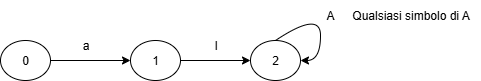
\includegraphics[width=0.5\textwidth]{images/esercizioautoma.png}
\end{center}
Con stato "2" come stato di accettazione.
\subsection{Automi deterministici e non deterministici}
\paragraph{Automa deterministico: } un automa è deterministico se e solo se la relazione di transizione è una funzione (quindi totale e univalente).
\paragraph{Automa non deterministico: } un automa è non deterministico se la relazione di transizione non è una funzione, ovvero c'è almeno uno stato in cui partono più di una transizione che ritornano lo stesso simbolo (non univalente) oppure c'è almeno uno stato a cui non sono collegate transizioni per tutti i simboli (non totale).

\subsection{Grammatiche}
Una \textbf{grammatica} è un insieme di regole che definisce come comporre le frasi di un linguaggio.\\
Una grammatica è una coppia $(S,P)$, con $S$ come insieme dei simboli non terminali e $P$ come insieme delle \textbf{produzioni}.
In una grammatica sono presenti simboli:
\begin{itemize}
    \item \textbf{Terminale:} simbolo considerato finale, che di per sè non allunga la stringa.
    \item \textbf{Non terminale:} simbolo che oltre ad un simbolo aggiunge altri simboli a scelta in posizioni ben precise.
\end{itemize}
Ogni regola di una grammatica si chiama \textbf{produzione} ed hanno la forma:
\[
Testa \rightsquigarrow Corpo 
\]
La testa è un simbolo terminale, il corpo una sequenza di simboli terminali e non. La freccia utilizzata nella definizione sopra è errata, quella giusta non è presente in Latex (quella giusta si chiama "potrebbe essere").
\paragraph{Albero di derivazione sintattica (Parse Tree): } albero che mostra la composizione di una stringa.\\\\
Non sempre esiste un automa a stati finiti in grado di definire una grammatica. Per esempio, questa grammatica non possiede un automa rappresentativo:
\[
\{a^nb^n | n \in N\} \text{ su alfabeto } A = \{a,b\}
\]

\section{Logica}
La \textbf{logica} è la disciplina che studia la correttezza.\\
Nella seconda metà del 1800 sono state sviluppate notazioni matematiche per gli operatori logici.\\
Tutto il calcolo dei computer si basa sulla logica.\\
La logica ci serve per esprimere concetti in modo non ambiguo.
\paragraph{Proposizione: } frase in linguaggio naturale che soffisfa:
\begin{itemize}
    \item \textbf{Prinipio del terzo escluso: } o è vera o è falsa
    \item \textbf{Principio di non contradditorietà: } non entrambi (vera e falsa)
\end{itemize}
Ogni proposizione è definita da una formula.\\
Quando una formula segue un modello si rappresenta così:
\[
\models P
\]
\paragraph{Tautologia: }formula proposizionale che è vera in ogni intepretazione, sono di modello:
\[
\models P
\]
\paragraph{Contraddizione: }formula proposizionale che è falsa in ogni interpretazione, sono di modello:
\[
\models \lnot P
\]
\paragraph{Conseguenza logica: } più formule (insieme $\Gamma$) convalidano un'altra formula, ovvero se tutte insieme seguono un modello:
\[
A \land B \text{ , } B \land C \models A \land C
\]
La dimostrazione valida per la conseguenza logica ($Q$ è dimostrabile da $\Gamma$ in $R$, ovvero l'insieme delle regole di inferenza) spiega che ogni formula in $\Gamma$:
\begin{itemize}
    \item O è un assioma / ipotesi in $\Gamma$ e quindi è vera.
    \item O è ottenuta tramite regole di inferenza, e quindi è vera.
\end{itemize}
\paragraph{Principio di sostituzione: } possono esistere regole "r" che dicono che se sono vere le formule $P_1,P_2,\ldots,P_n$ allora è vera P:
\[
\frac{P_1 \ldots P_n}{P}[r]
\]
Esistono delle formule vere \textbf{a prescindere}, sempre, si chiamano \textbf{assiomi}.
\[
\frac{}{P_1}[r]
\]
Ogni \textbf{proof system} può essere \textbf{completo}, ma è sempre \textbf{corretto}:
\begin{itemize}
    \item \textbf{Corretto: }$\Gamma \vdash _R P \implies \Gamma \models P$
    \item \textbf{Completo: }$\Gamma \models P \implies \Gamma \vdash _R$
\end{itemize}
Quando due formule / formule proposizionali sono \textbf{logicamente identiche} (hanno lo stesso output per ogni input) si indica cosi:
\[
P1 \equiv P2
\]
\subsection{Tecniche di dimostrazione}
\paragraph{Contronominale: } dimostrazione dell'inverso della tesi (tutto col not)
\paragraph{Dimostrazione per assurdo: } dimostrazione che la tesi non può non essere vera o che il contrario della tesi è sempre falso
\subsection{Logica dei predicati}
"Se Anna è la mamma di Bruno e Bruno ha figli, allora Anna è nonna"\\
Questa è una proposizione, ma nel linguaggio matematico / logico è difficile realizzarlo, possiamo fare cosi:
\[
\text{mamma(Anna,Bruno) } \land \text{ haFigli(Bruno) } \implies \text{ nonna(Anna)}
\]
Queste "funzioni" che ritornano Intuitivamente solo valori booleani si chiamano \textbf{predicati}.
\paragraph{Quantificatori:} simboli che indicano pronomi o aggettivi come "tutti","nessuno","alcuni"...\\
Indicano le quantità.
\[
\forall = \text{ per ogni (tutti)}
\]
\[
\exists = \text{ esiste (almeno 1, alcuni)}
\]
\[
\nexists = \text{ non esiste (nessuno)}
\]
L'uso dei quantificatori $Q$ assume questa forma:
\[
Qx . P \text{ oppure } Qx : P
\]
Con P come formula proposizionale.
\paragraph{Alfabeti del primo ordine:} un alfabeto del primo ordine $A$ è una quadrupla $(C,F,P,V)$ dove:
\begin{itemize}
    \item $C = $ costanti (Anna, Bruno...)
    \item $F = $ funzioni (padre, altezza... (input: dominio, output: dominio))
    \item $P = $ predicati (input: dominio, output: bool)
    \item $V = $ variabili (x,y,pippo...)
\end{itemize}
\end{document}
